\documentclass[english,floatsintext,man]{apa6}

\usepackage{amssymb,amsmath}
\usepackage{ifxetex,ifluatex}
\usepackage{fixltx2e} % provides \textsubscript
\ifnum 0\ifxetex 1\fi\ifluatex 1\fi=0 % if pdftex
  \usepackage[T1]{fontenc}
  \usepackage[utf8]{inputenc}
\else % if luatex or xelatex
  \ifxetex
    \usepackage{mathspec}
    \usepackage{xltxtra,xunicode}
  \else
    \usepackage{fontspec}
  \fi
  \defaultfontfeatures{Mapping=tex-text,Scale=MatchLowercase}
  \newcommand{\euro}{€}
\fi
% use upquote if available, for straight quotes in verbatim environments
\IfFileExists{upquote.sty}{\usepackage{upquote}}{}
% use microtype if available
\IfFileExists{microtype.sty}{\usepackage{microtype}}{}

% Table formatting
\usepackage{longtable, booktabs}
\usepackage{lscape}
% \usepackage[counterclockwise]{rotating}   % Landscape page setup for large tables
\usepackage{multirow}		% Table styling
\usepackage{tabularx}		% Control Column width
\usepackage[flushleft]{threeparttable}	% Allows for three part tables with a specified notes section
\usepackage{threeparttablex}            % Lets threeparttable work with longtable

% Create new environments so endfloat can handle them
% \newenvironment{ltable}
%   {\begin{landscape}\begin{center}\begin{threeparttable}}
%   {\end{threeparttable}\end{center}\end{landscape}}

\newenvironment{lltable}
  {\begin{landscape}\begin{center}\begin{ThreePartTable}}
  {\end{ThreePartTable}\end{center}\end{landscape}}




% The following enables adjusting longtable caption width to table width
% Solution found at http://golatex.de/longtable-mit-caption-so-breit-wie-die-tabelle-t15767.html
\makeatletter
\newcommand\LastLTentrywidth{1em}
\newlength\longtablewidth
\setlength{\longtablewidth}{1in}
\newcommand\getlongtablewidth{%
 \begingroup
  \ifcsname LT@\roman{LT@tables}\endcsname
  \global\longtablewidth=0pt
  \renewcommand\LT@entry[2]{\global\advance\longtablewidth by ##2\relax\gdef\LastLTentrywidth{##2}}%
  \@nameuse{LT@\roman{LT@tables}}%
  \fi
\endgroup}


  \usepackage{graphicx}
  \makeatletter
  \def\maxwidth{\ifdim\Gin@nat@width>\linewidth\linewidth\else\Gin@nat@width\fi}
  \def\maxheight{\ifdim\Gin@nat@height>\textheight\textheight\else\Gin@nat@height\fi}
  \makeatother
  % Scale images if necessary, so that they will not overflow the page
  % margins by default, and it is still possible to overwrite the defaults
  % using explicit options in \includegraphics[width, height, ...]{}
  \setkeys{Gin}{width=\maxwidth,height=\maxheight,keepaspectratio}
\ifxetex
  \usepackage[setpagesize=false, % page size defined by xetex
              unicode=false, % unicode breaks when used with xetex
              xetex]{hyperref}
\else
  \usepackage[unicode=true]{hyperref}
\fi
\hypersetup{breaklinks=true,
            pdfauthor={},
            pdftitle={Vestibular Contributions to Spatial Perspective Transformations: From Sensory Inference To Imagined Self-Motion},
            colorlinks=true,
            citecolor=blue,
            urlcolor=blue,
            linkcolor=blue,
            pdfborder={0 0 0}}
\urlstyle{same}  % don't use monospace font for urls

\setlength{\parindent}{0pt}
%\setlength{\parskip}{0pt plus 0pt minus 0pt}

\setlength{\emergencystretch}{3em}  % prevent overfull lines

\ifxetex
  \usepackage{polyglossia}
  \setmainlanguage{}
\else
  \usepackage[english]{babel}
\fi

% Manuscript styling
\captionsetup{font=singlespacing,justification=justified}
\usepackage{csquotes}
\usepackage{upgreek}

 % Line numbering
  \usepackage{lineno}
  \linenumbers


\usepackage{tikz} % Variable definition to generate author note

% fix for \tightlist problem in pandoc 1.14
\providecommand{\tightlist}{%
  \setlength{\itemsep}{0pt}\setlength{\parskip}{0pt}}

% Essential manuscript parts
  \title{Vestibular Contributions to Spatial Perspective Transformations: From
Sensory Inference To Imagined Self-Motion}

  \shorttitle{Vestibular Contributions to SPT}


  \author{Andrew W. Ellis~\& Fred W. Mast}

  \def\affdep{{"", ""}}%
  \def\affcity{{"", ""}}%

  \affiliation{
    \vspace{0.5cm}
          \textsuperscript{} Department of Psychology, University of Bern, Switzerland  }

  \authornote{
    \newcounter{author}
    Andrew W. Ellis \& Fred W. Mast, Department of Psychology. AE and FM
    planned and conducted the research; AE and FM analyzed the data and
    wrote the manuscript. Code for simulations is available at
    \url{https://osf.io/u26mq}.

                      Correspondence concerning this article should be addressed to Andrew W. Ellis, Fabrikstrasse 8, 3012 Bern, Switzerland. E-mail: \href{mailto:andrew.ellis@psy.unibe.ch}{\nolinkurl{andrew.ellis@psy.unibe.ch}}
                          }


  \abstract{Recent research has indicated that the vestibular network is involved in
various cognitive tasks involving mental spatial transformations.
However, the nature of this involvement remains unclear. Here, we
provide a computational framework for vestibular cognition and discuss
this in the context of perspective transformations, which require a
simulated rotation of the self. We explore how the ability to model the
effects of body rotation using vestibular input might enable the ability
to imagine body rotations. We approach this problem by extending
previous models of vestibular sensory processing to include the ability
to model the sensory consequences of self-initiated movements, and
discuss how this can be further extended to allow mentally simulated
rotations of the self. We \ldots{} Predicting the sensory input is key
to understanding imagined rotations. Mental imagery goes beyond
prediction, rather, it involves the use of counterfactual queries in a
probabilistic model.}
  \keywords{probabilistic graphical models, particle filter, embodied cognition,
vestibular cognition, spatial perspective taking, mental imagery \\

    \indent Word count: X
  }

\usepackage[titles]{tocloft}
\cftpagenumbersoff{figure}
\renewcommand{\cftfigpresnum}{\itshape\figurename\enspace}
\renewcommand{\cftfigaftersnum}{.\space}
\setlength{\cftfigindent}{0pt}
\setlength{\cftafterloftitleskip}{0pt}
\settowidth{\cftfignumwidth}{Figure 10.\qquad}

\cftpagenumbersoff{table}
\renewcommand{\cfttabpresnum}{\itshape\tablename\enspace}
\renewcommand{\cfttabaftersnum}{.\space}
\setlength{\cfttabindent}{0pt}
\setlength{\cftafterloftitleskip}{0pt}
\settowidth{\cfttabnumwidth}{Table 10.\qquad}


  \usepackage{caption}

\usepackage{amsthm}
\newtheorem{theorem}{Theorem}
\newtheorem{lemma}{Lemma}
\theoremstyle{definition}
\newtheorem{definition}{Definition}
\newtheorem{corollary}{Corollary}
\newtheorem{proposition}{Proposition}
\theoremstyle{definition}
\newtheorem{example}{Example}
\theoremstyle{remark}
\newtheorem*{remark}{Remark}
\begin{document}

\maketitle

\setcounter{secnumdepth}{0}



% pandoc-xnos: macro to create a caption without a prefix
\makeatletter
\long\def\@makenoprefixcaption#1#2{
  \vskip\abovecaptionskip
  \sbox\@tempboxa{#2}
  \ifdim \wd\@tempboxa >\hsize
    #2\par
  \else
    \global \@minipagefalse
    \hb@xt@\hsize{\hfil\box\@tempboxa\hfil}
  \fi
  \vskip\belowcaptionskip}
\makeatother

% pandoc-fignos: save original macros
\makeatletter
\let\@oldmakecaption=\@makecaption
\let\oldthefigure=\thefigure
\let\oldtheHfigure=\theHfigure
\makeatother

% pandoc-fignos: environment disables figure caption prefixes
\makeatletter
\newcounter{figno}
\newenvironment{no-prefix-figure-caption}{
  \let\@makecaption=\@makenoprefixcaption
  \renewcommand\thefigure{x.\thefigno}
  \renewcommand\theHfigure{x.\thefigno}
  \stepcounter{figno}
}{
  \let\thefigure=\oldthefigure
  \let\theHfigure=\oldtheHfigure
  \let\@makecaption=\@oldmakecaption
  \addtocounter{figure}{-1}
}
\makeatother

% pandoc-xnos: cleveref fakery
\newcommand{\plusnamesingular}{}
\newcommand{\starnamesingular}{}
\newcommand{\xrefname}[1]{\protect\renewcommand{\plusnamesingular}{#1}}
\newcommand{\Xrefname}[1]{\protect\renewcommand{\starnamesingular}{#1}}
\providecommand{\cref}{\plusnamesingular~\ref}
\providecommand{\Cref}{\starnamesingular~\ref}
\providecommand{\crefformat}[2]{}
\providecommand{\Crefformat}[2]{}

% pandoc-xnos: cleveref formatting
\crefformat{figure}{Figure~#2#1#3}
\Crefformat{figure}{Figure~#2#1#3}

\section{Introduction}\label{introduction}

Adopting the spatial perspective of another person is generally
considered an essential cognitive ability, and plays a vital role in our
ability to determine what another person can see and in order to
coordinate joint actions (Creem-Regehr, Gagnon, Geuss, \& Stefanucci,
2013, Pezzulo, Iodice, Ferraina, \& Kessler (2013)). Many studies have
also pointed out that perspective taking is of fundamental importance
for language comprehension and communication (Beveridge \& Pickering,
2013), and social cognition in general (Deroualle \& Lopez, 2014).

A number of recent studies have demonstrated that the vestibular system,
which deals with sensory signal relating to movements of the head, is
involved in such spatial transformations (Lenggenhager, Lopez, \&
Blanke, 2008, Deroualle, Borel, Devèze, \& Lopez (2015), Falconer \&
Mast (2012), Gardner, Stent, Mohr, \& Golding (2016)). This is
demonstrated in the form of interference effects between mental
transformations and concurrent sensory stimulation. However, to date,
there has little attempt to understand the involvement of the vestibular
system in higher-level cognitive abilities from a computational
perspective. In this paper, we focus specifically on the role of the
vestibular system for spatial perspective transformations, and we draw
the link between probabilistic computations performed by the vestibular
system in the service of real-time interaction with the world, and the
brain's ability to run mental simulations for the purpose of adopting
the perspective of another person.

Consider the use of deictic pronouns, such as \enquote{this} or
\enquote{that} and \enquote{left} or \enquote{right}. These terms only
assume a their meaning when placed within a certain frame of reference
(FOR). For example, in a dialogue between two speakers, the statement
\enquote{I would like that one}, or \enquote{I would like the one on the
right} can only be understood under the assumption that the deictic
terms \enquote{that} and \enquote{right} are used in an egocentric FOR.
In addition, both interlocutors must be able to access the other's FOR
with respect to an external FOR. In other words: In order to give
instructions, the speaker must be able to mentally assume the
addressee's position in space. A further example that requires a similar
spatial transformation is when two people want to perform a coordinated
action, such as lifting a heavy object. This requires having knowledge
of the other's potential actions in order to adjust one's own actions,
and this again requires knowledge of the other's position with an
external FOR. A judgement about what kind of actions the other person
can perform requires an embodied simulation using a representation of
one's own body schema (Pezzulo et al., 2013). Giving an instruction to
another person thus requires running an embodied simulation in order to
infer what kind of motor commands the other person should perform
\textbf{{[}Blakemore and Decety, 2001; Wolpert et al., 2003; Jeannerod,
2006; Pezzulo et al., 2007, 2013; Dindo et al., 2011; Pezzulo,
2011a,b{]}}. This embodied simulation is performed using one's own body
schema. Communicating this information to the other actor requires
knowing the position of the addressee's FOR relative to the external
reference frame, and the difference between the speaker and the
addressee's egocentric reference frames. Perspective taking thus can be
conceived of as a aligning a representation of one's body with that of
another person in order to access spatial information from a viewpoint
other than one's own egocentric viewpoint. In order to achieve this
alignment, one must perform translations and rotations of one's own
egocentric reference frame. Processing translations and rotations of the
head and body is the core domain of the vestibular system, and thus is
of particular interest for research into mental spatial transformations.
Spatial transformations in 6 dimensions (translation along 3 axes, and
rotations around 3 axes) are highly complex, and non-linear, and we
propose that the brain adopts the strategy of simulating motion of the
body through space in order achieve a desired target position. This
effectively amounts to a running a simulation of dynamical system,
consisting of simulated limb movements and the resulting sensory
consequences. \autoref{fig:spt-schematic} (a) shows a simple scenario in
which a speaker wants to give an addressee, standing opposite, verbal
instructions about an action to perform on an external object. The
speaker must determine the most suitable action, given the addressee's
position relative to the external object, and in order to achieve this
goal, the speaker must align himself with the addressee, so that he can
use his own body-centred reference frame to quickly simulate the best
action. In this example, alignment with the addressee's reference frame
consists of a forwards translation and a rotation around the vertical
axis. This can be described as an imagined movement, in which the goal
is achieve a specific position.

\begin{figure}
\centering
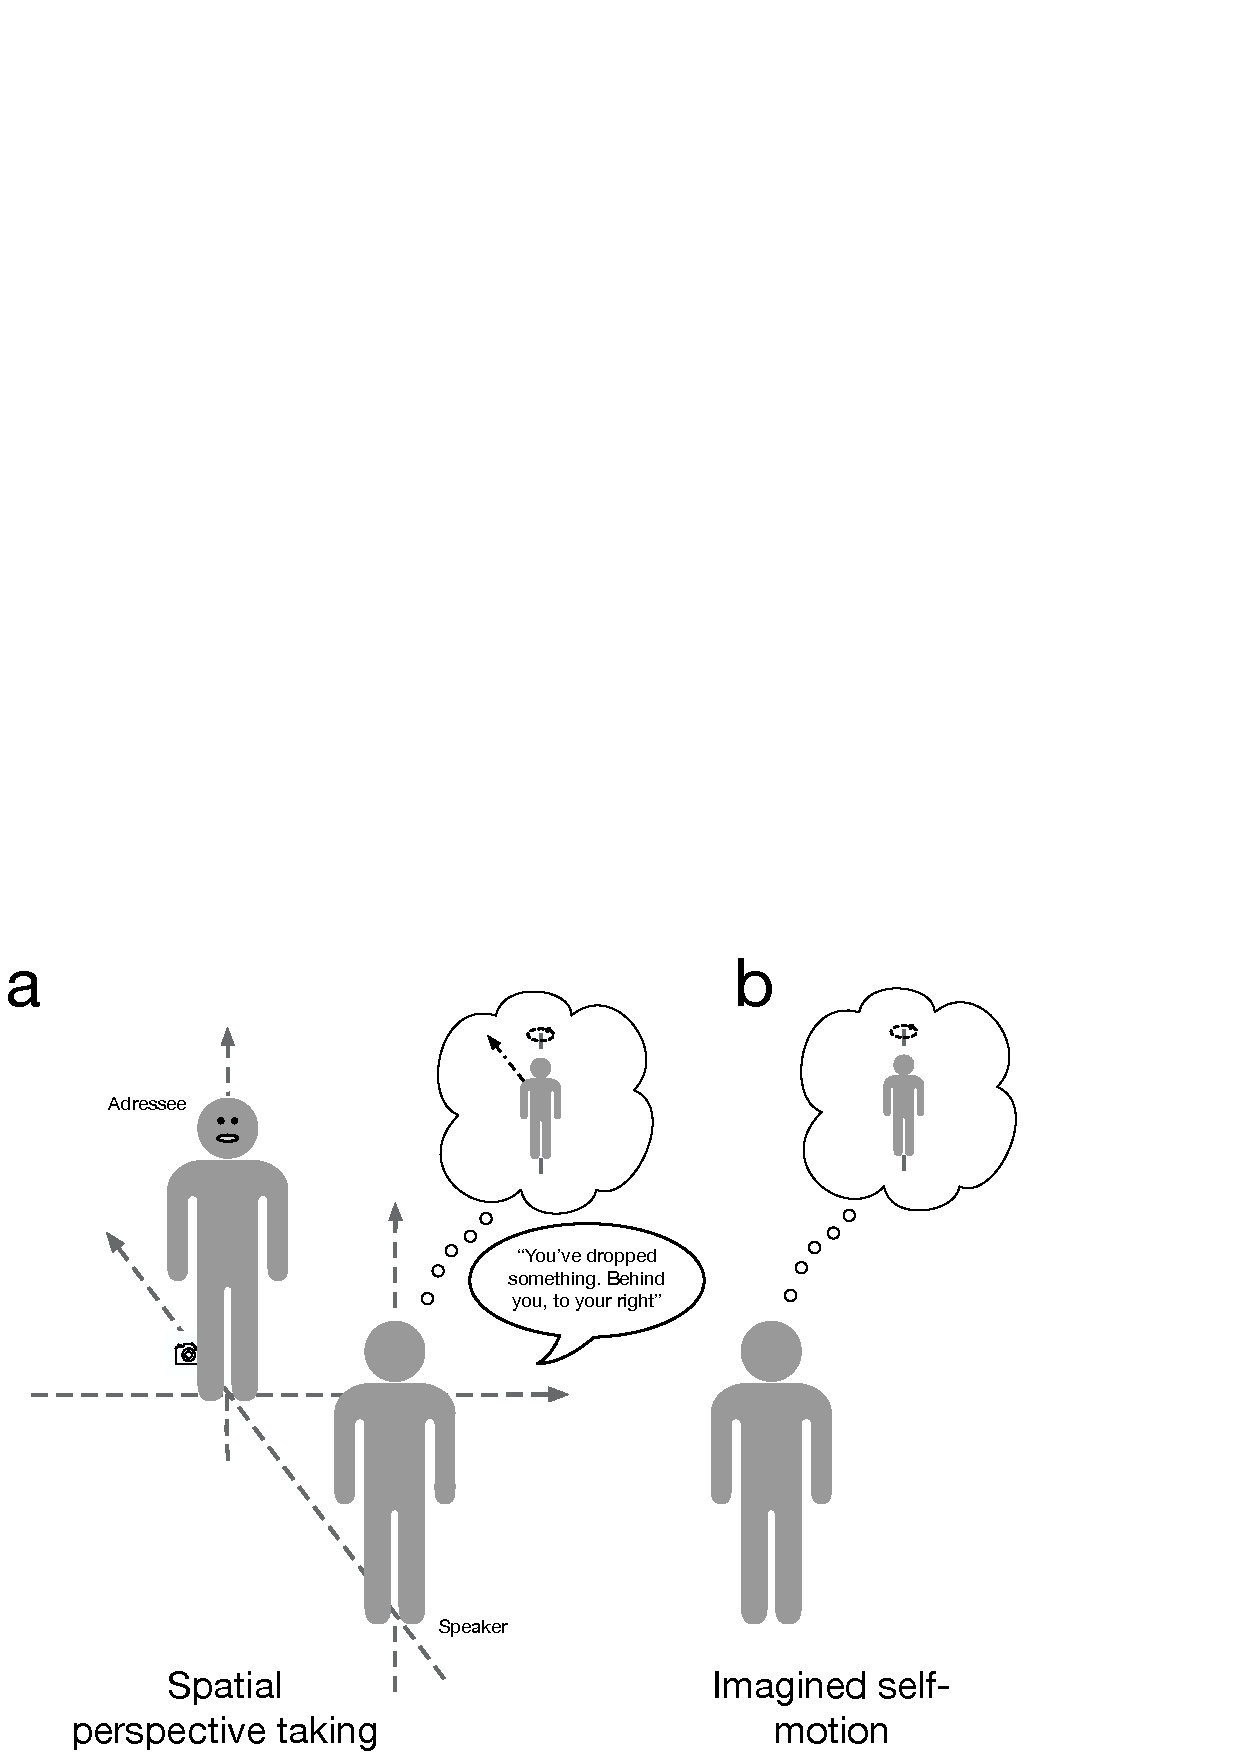
\includegraphics[width=0.50000\textwidth]{diagrams/fig-1-common-process.pdf}
\caption{Perspective taking and imagined self-motion involve spatial
transformations of a representation of the self. (a) If a speaker's goal
is to take the perspective of an addressee, he must first solve the
inverse problem of determining the appropriate action, and then run a
forwards simulation in order to perform a translation and rotation of
his own egocentric reference frame. These operations can be viewed as
imagined movements.(b) Focussing on imagined rotation around the
vertical axis allows us to simplify the problem, and highlights the fact
that perspective taking and mental imagery involve common
computations.\label{fig:spt-schematic}}
\end{figure}

In order to do this, the speaker must first determine what type of
movement to perform, and the direction, velocity and duration that lead
to the desired outcome. This means that in order to know what to
simulate, the speaker must first work backwards from the desired
outcome, and infer the actions that are most likely to lead to that
outcome. This is known in the field of motor control as the inverse
problem (Wolpert \& Kawato, 1998). In order to achieve the desired
position, the motor commands can then be simulated, and the expected
sensory consequences can be estimated; this is known as the forward
problem. \xrefname{Figure}\cref{fig:spt-schematic} (b) shows that if the
goal is to simply simulate the perceptual experience of rotation around
the body's vertical (yaw) axis, rather than project a representation of
one's body onto a target, the problem is simplified; the actor can
perform forward inference without the need to determine the optimal
motor action. As demonstrated by Penny, Zeidman, \& Burgess (2013),
these computations can be performed in a common probabilistic model.
Interestingly, this has been discussed in the context of reinforcement
learning, and planning in humans has been described as reverse inference
(Botvinick \& Toussaint, 2012). Further, (Pickering \& Clark, 2014)
discuss the relationship between control-theoretic notions of
inverse/forward models, known collectively as internal models, and and
more general concepts of a generative model in a hierarchical Bayesian
framework.

Performing a simulation of body movements and estimating the sensory
consquences amounts to simulating the behaviour of a dynamical system;
this requires a generative model of the system. The aim of this paper is
to specifically investigate the generative model that may be used for
mental spatial transformations. The ability to run embodied simulations
is often claimed to be grounded in the relevant sensorimotor circuits,
and we claim that the vestibular system is ideally suited to investigate
this connection, because the generative models used by the vestibular
system for dynamic sensory inference have been extensively investigated
using approaches from optimal control theory, and more recently, dynamic
Baysian inference. The vestibular system faces a number of challenges in
interpreting the sensory measurements provided by the semi-circular
canals (SCC) and otolith organs. On the one hand, these signals are very
noisy, and ambiguous (MacNeilage, Ganesan, \& Angelaki, 2008); the
otoliths respond both to translations and tilt of the head relative to
gravity, and in order to disambiguate between translation and tilt, the
brain must perform sophisticated computations at the level of the brain
stem. It has become clear that the nature of these computations is
probabilistic, and that the brain makes use of strong prior beliefs in
order to interpret these sensory signals. A further challenge faced by
the vestibular system is that it needs to distinguish between sensory
signals that are the result of active motion, and those resulting from
external forces (Cullen, Brooks, \& Sadeghi, 2009, Cullen (2014)). The
ability to distinguishing re-afferent from ex-afferent sensory signals
is an essential capability of all organisms that move actively (Crapse
\& Sommer, 2008).

Furthermore, the apparent connection between mental imagery and
predictive processing has repeatedly been alluded to (Moulton \&
Kosslyn, 2009, Clark (2012), Gambi \& Pickering (2015)), and Grush
(2004) claims that mental imagery is performed by emulator circuits
implementing a forward model. These ideas can also be addressed from a
computational point of view in the context of dynamic Bayesian
inference, where there are multiple roles for sensory predictions, over
different time scales. This was recently discussed by (Tian \& Poeppel,
2012) in the context of imagined speech.

We proceed by introducing recent models of Bayesian inference for
real-time, dynamic sensory processing of vestibular data, based on
particle filters (Laurens \& Droulez, 2007, Karmali \& Merfeld (2012)),
and we reframe these as probabilistic graphical models. This allows us
to investigate the generative model separately from the algorithm used
for inference, and we then extend the basic model for sensory inference
in order to provide the ability to model the consequences of
self-initiated, active movements. Our aims are to:

\begin{enumerate}
\def\labelenumi{\arabic{enumi})}
\tightlist
\item
  identify various forms of predictive processing in the context of
  dynamic sensory processing.
\item
  identify various sources of interference between higher-level
  cognition and lower-level sensory processing.
\item
  provide suggestions for future research aiming to investigate the
  connections between cognitive and sensory processing.
\end{enumerate}

\section{Dynamic Bayesian models for sensory
inference}\label{dynamic-bayesian-models-for-sensory-inference}

\subsection{Previous work}\label{previous-work}

Whereas early models of vestibular sensory processing were inspired by
control theory (Borah, Young, \& Curry, 1988, Merfeld, Zupan, \& Peterka
(1999)), several recent studies have described vestibular sensory
processing as dynamic Bayesian inference (Laurens \& Droulez, 2007,
MacNeilage et al. (2008), Karmali \& Merfeld (2012)). Selva \& Oman
(2012) provide a recent review of the relationship between optimal
observer models and models which employ Kalman filtering, and show that
these are largely equivalent. Both Karmali \& Merfeld (2012) and Laurens
\& Droulez (2007) described vestibular sensory inference in terms of
particle filtering, which is a particular inference algorithm that can
be used to perform inference in state-space models. (Doucet, Godsill, \&
Andrieu, 2000, Doucet \& Johansen (2009)). Using their model, Laurens \&
Droulez (2007) were able to simulate perceptual responses to
centrifugation and off-vertical axis rotations.

A further well-known phenomenon of vestibular perception is velocity
storage, which is defined as the slower decay of perceptual and
oculomotor responses, relative to the SCC afferent responses (Raphan,
Matsuo, \& Cohen, 1979), \textbf{{[}Robinson 1977{]}}. This is generally
seen as evidence for the existence of an internal model in the
processing of vestibular signals. Karmali \& Merfeld (2012) focussed on
one-dimensional angular velocity during yaw rotations; their model was
able to explain the phenomenon of velocity storage as a consequence of
particle filtering, with the time constant of velocity storage depending
on the variability of the sensory afferent signals.

\subsection{Generative model for sensory
inference}\label{generative-model-for-sensory-inference}

We proceed by providing a brief introduction to the concept of
state-space models, and particle filtering, which is a particular
algorithm that can perform inference in state-space models. While Kalman
filters are restricted to linear Gaussian State-space models, particle
filtering can be applied to arbitrary nonlinear models. State-space
models can be seen as special cases of more general Bayesian
hierarchical models (Bishop, 2006; Murphy, 2012). Following the same
approach as Penny et al. (2013), we first describe the generative model
used for sensory inference as a dynamic probabilistic graphical model.

A state-space is special case of a dynamic latent variable model which
is suitable for modelling dynamical system in terms of latent,
unobservable processes and noisy observations. As an example, consider
the case where we want to model the velocity and position during a
leftward head turn. While the SCC measures angular acceleration, the
afferent signals are thought to be proportional to the angular velocity
of the head with a frequency band of approximately 0.1 -- 10 Hz, which
constitutes the range of natural head movements (Carriot, Jamali,
Chacron, \& Cullen, 2014; Grabherr, Nicoucar, Mast, \& Merfeld, 2008).
The measurements are observations of the true, unobservable angular
velocity; however, they are contaminted by Gaussian noise, which is
determined by characteristics of the sensory organs.
\autoref{fig:head-turn-data} shows a sequence of noisy measurements
during a two-second turn of the head. The acceleration generating the
movement is sinusoidal, given for each time step \(t\) by
\(Asin(2\pi t/T)\), where \(A\) is the amplitude of the movement,
\(T = 1/f\) is the duration of the movement, and \(f\) is the frequency.
This acceleration results in a peak velocity \(\omega_{peak} = AT/\pi\)
and a final angular position \(\theta_{final} = AT^2/2\pi\).

\begin{no-prefix-figure-caption}

\begin{figure}
\centering
\includegraphics{../generated-figures/head-turn-data-1.pdf}
\caption{\label{fig:head-turn-data}Sensory measurements obtained during a
short head turn. The goal is to infer the latent angular velocity and
position, based on the noisy measurements. \label{fig:head-turn}}
\end{figure}

\end{no-prefix-figure-caption}

The key idea is that we can write model the dynamics of a system by the
evolution of the latent state variables in discrete time steps as a
Markov process, where the state at each time point \(t\) depends only on
the previous state at time \(t-1\). This is referred to as the process
model. Estimating the velocity \(\omega\) and position \(\theta\) in
discrete time therefore requires writing the kinematic equations as a
set of first order difference equations.

\[\theta_t = \theta_{t-1} + \omega_{t-1} \Delta t\]
\[\omega_{t} = \omega_{t-1}\]

Note that we have omitted the acceleration from the process model, for
the sake of simplicity; this amounts to assuming a constant velocity
model. These kinematic equations form a linear model, and could
optionally be written in matrix notation. For further simplicity, we
retain the current notation. Next, we consider the measurements at each
time step \(t\) as depending only on the current state. This simply
implements the idea that the sensory signal depends only on the current
head velocity. The above equations represent the expected values of the
state and observation variables. In order to complete the generative
model, we require a description of the stochastic nature dependancies.
We model both process and measurement noise a being normally
distributed, leading to the following linear Gaussian state-space model:

\[x_t = f(x_{t-1}, \epsilon)\] \[y_{t} = g(x_t, \delta)\]
\[\epsilon \sim N(0, \sigma^2_\epsilon) \]
\[\delta \sim N(0, \sigma^2_\delta) \]

where the state variable \(x_t\) consists of both the velocity
\(\omega_t\) and position \(\theta_t\), and \(y_{t}\) denotes the
sensory measurement.\footnote{Note that we although both Laurens \&
  Droulez (2007), Karmali \& Merfeld (2012) consider a realistic sensor
  model, for simplicity, we implement the sensor as being a noisy
  realisation of the velocity. Our model is not intended to be a
  realistic model of the SCC; rather, we focus on the probabilistic
  computations.} \(\epsilon\) and \(\delta\) are zero-mean Gaussian
noise terms with variances \(\sigma^2_\epsilon\) and
\(\sigma^2_\delta\). These refer to the process and measurement noise,
respectively. The process noise

\autoref{fig:graphical-model-inference} shows a representation of
state-space model as a graphical model, unrolled over multiple time
steps. Starting at time 0, the state variables evolve according to the
process model, with the measurements at each time step being generated
according to the measurement model. The 2-dimensiontal latent state
variable is unshaded, to indicate that it cannot be observed, wheres the
observed sensory measurements are shaded. Whereas previous models were
discussed in terms of the particular filtering algorithm used, the
graphical notation highlights the fact that a state-space model can be
viewed as a dynamic latent factor model (Blei, 2014). This opens up the
possibility of extending the graphical model to include higher-level
variables. After discussing particle filtering, an inference algorithm
often used to infer the values of the latent state variables, we will
introduce our extension to the model that will allow a prediction of the
consequences of active movements.

\begin{figure}
\includegraphics[width=1\linewidth]{diagrams/dynamic-belief-network-inference-1} \caption{Graphical model for inferring the 2-dimensional state $x$, consisting of angular velocity and position, based on noisy sensory measurements $y$.}\label{fig:graphical-model-inference}
\end{figure}

\subsection{Particle filtering}\label{particle-filtering}

We give a brief overview of particle filtering, concentrating on those
aspects most relevant for this study. For a more thorough treatment, see
Doucet et al. (2000) and Doucet \& Johansen (2009). Speekenbrink (2016)
provides a recent review with applications in psychological research.
Particle filtering is an algorithm for performing approximate Bayesian
inference in a graphical model. It proceeds by recursively computing the
distribution of the current state \(x_t\) as a a function of its parent
nodes, consisting in our example of the state at the previous time step.

The general procedure for recursive Bayesian inference is to perform
alternating prediction and updating steps.

\begin{enumerate}
\def\labelenumi{\arabic{enumi})}
\item
  Predict step: At time t, the current state is predicted according to
  the process model. This prediction is maintained in the form of
  probability distributions over all the values.
\item
  Update step: a measurement is obtained, and this measurement is used
  in order to update the state estimate.
\end{enumerate}

By recursively estimating the current state, the observations can be
processed continuously; thus, the agent does not need to store the
entire history of observations -- only the previous belief state
estimate and the current observation are needed in order to estimate the
current state. At time step t, the agent observes the value of , and
this observation is used to update the previous belief:

\autoref{fig:particle-filter-explained} shows a diagram \ldots{}

\begin{figure}
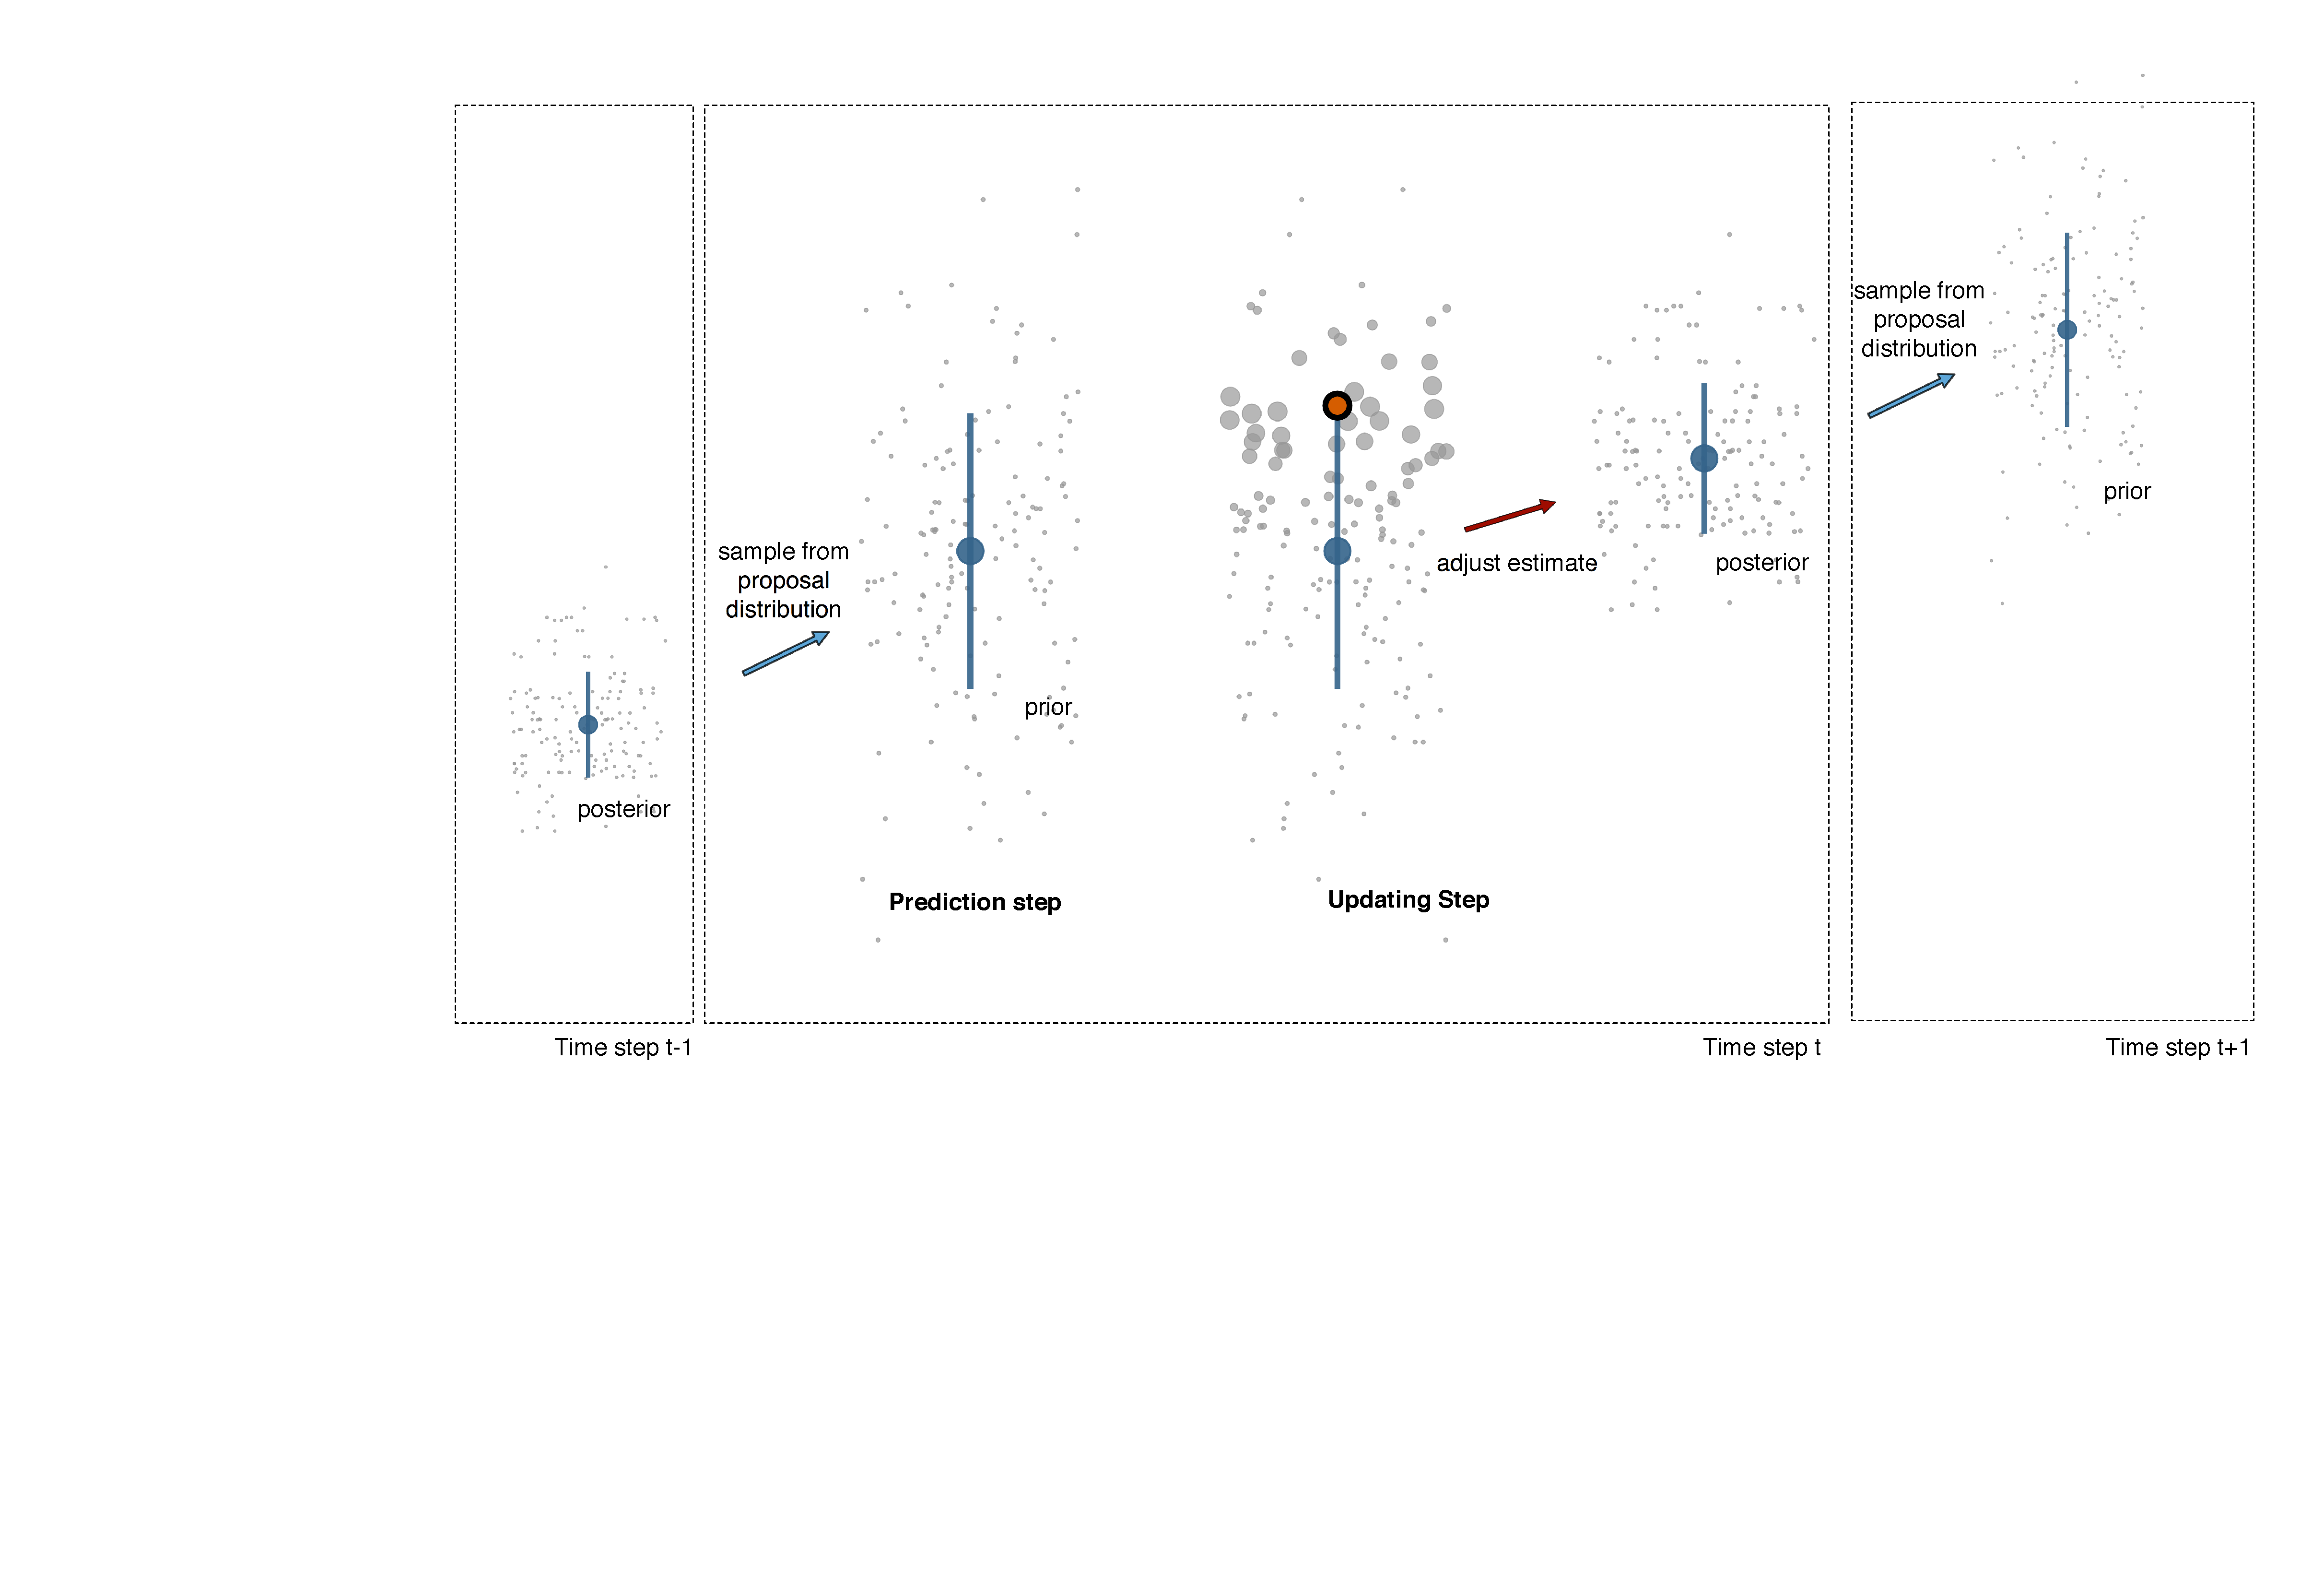
\includegraphics[width=1\linewidth]{diagrams/figure-particle-filter-explained} \caption{Particle filter computations performed at every time step. The cloud of particles (grey circles) represents the current belief state. Initially, a prediction is made for each particle by sampling from the proposal distribution, which is determined by the agent’s kinematic model. This is equivalent to sampling from the prior distribution. Then, during the updating step, an observation  is obtained (shown as a black diamond). Each particle is assigned an importance weight, according to how well it explains the observation. Each particle's diameter reflects its importance weight. Subsequently, a new set of particles is formed by weighted multinomial resampling, with each particle's probability of being chosen proportional to its importance weight. The particle cloud's mean and standard deviation are shown as light grey circles and lines. This resulting cloud of particles represents the posterior distribution. This posterior subsequently forms the prior distribution for the next time step.}\label{fig:particle-filter-explained}
\end{figure}

\autoref{fig:passive} shows the estimated velocity \ldots{}

\begin{no-prefix-figure-caption}

\begin{figure}
\centering
\includegraphics{../generated-figures/passive-1.pdf}
\caption{\label{fig:passive}Particle filter applied\ldots{}}
\end{figure}

\end{no-prefix-figure-caption}

\subsection{Summary}\label{summary}

\section{Extend previous models with control
input}\label{extend-previous-models-with-control-input}

For sensory inference of a passive disturbance, the algorithm can be run
with fixed parameters. Here we extend the basic particle filtering
(algorithm) model, in order to:

\begin{itemize}
\tightlist
\item
  \textbf{provide the capability to model the sensory consequences of
  self-initiated actions} (i.e.~predict/infer the consequences of one's
  own actions)
\item
  provide the capability to run a Monte Carlo simulation using the same
  generative model as is used for sensory inference
\end{itemize}

\subsection{Generative Model}\label{generative-model}

The generative model is a state-space model, which itself is a dynamic
model consisting of latent (state variables) and observed (measured)
variables.

\subsection{Inference Algorithm}\label{inference-algorithm}

Sequential Monte Carlo

\section{Modelling questions}\label{modelling-questions}

Experimental results to be explained: Wertheim, Mesland, \& Bles (2001)
report a cognitive suppression of otolith responses, based on
participants' prior beliefs about possible motions.

\section{An Investigation of Various
Priors}\label{an-investigation-of-various-priors}

Here, we identify the various forms of predictive processing in the
context of real-time sensory inference using SMC \#\# Related to
Filtering Algorithm \#\# Higher-level Priors control input
-\textgreater{} infer the consequences of one's own actions.

\section{Various sources of
interference}\label{various-sources-of-interference}

Here, we identify various sources of intereference (2-way) between
thought (higher-level cognition) and lower-level sensory processing

\subsection{Model mis-specification}\label{model-mis-specification}

If an observer uses a strong higher level prior, i.e.~the wrong
direction, this means that the data may be completely mis-interpreted.
(call this: the effect of inappropriate priors (Schwabe \& Blanke,
2008))

\subsection{Re-use of same generative
model}\label{re-use-of-same-generative-model}

This may lead to leakage, i.e.~inadvertently incorporating sensory
evidence

\subsection{Decision-making}\label{decision-making}

The interference may be explained in terms of higher-level perceptual
decision -making mechanisms \#\# evidence accumulation \#\# bias
(Starting point)

\subsection{Summary}\label{summary-1}

Interference may the result of either inappropriate priors, leading to a
mis-specified filtering algorithm, or biased decision-making. We should
be able to investigate which by applying cognitive process models that
explain response times and choices.

\section{Simulations}\label{simulations}

\section{General Discussion}\label{general-discussion}

The main result of this study is - place the emerging field of
vestibular cognition with a framewotk for dynamic probabilistic
inference and draw links to established models of sensory processing -
interpret result from vestibular cognition studies showing interference
between thought and perception as being the result of biased sensory
processing

\subsection{A comparison with previous
models}\label{a-comparison-with-previous-models}

Unfortunately, there aren't many, but see (Hiatt, Trafton, Harrison, \&
Schultz, 2004): imagined motion through space vs.~rotating contents of
visual buffer

\subsection{Support for our model:
Nigmatullina}\label{support-for-our-model-nigmatullina}

\subsection{Neuronal implementation}\label{neuronal-implementation}

(Lopez \& Blanke, 2011; Lopez, Blanke, \& Mast, 2012) (Klingner, Axer,
Brodoehl, \& Witte, 2016) (Eulenburg, Müller-Forell, \& Dieterich, 2012)

\subsubsection{Sensory gating}\label{sensory-gating}

(Gale et al., 2016)

\subsubsection{Head direction cells}\label{head-direction-cells}

Why dynamic simulation? Maybe in order to provide vestibular in put to
head direction cells (Taube, 2007)

\section{Summary and conclusions}\label{summary-and-conclusions}

\section{Acknowledgements}\label{acknowledgements}

\section{Motion Data}\label{motion-data}

\section{Tables}\label{tables}

\begin{longtable}[]{@{}rlcl@{}}
\caption{Demonstration of simple table syntax.}\tabularnewline
\toprule
Right & Left & Center & Default\tabularnewline
\midrule
\endfirsthead
\toprule
Right & Left & Center & Default\tabularnewline
\midrule
\endhead
12 & 12 & 12 & 12\tabularnewline
123 & 123 & 123 & 123\tabularnewline
1 & 1 & 1 & 1\tabularnewline
\bottomrule
\end{longtable}

\begin{longtable}[]{@{}clrl@{}}
\caption{Here's the caption. It, too, may span multiple
lines.}\tabularnewline
\toprule
\begin{minipage}[b]{0.15\columnwidth}\centering\strut
Centered Header\strut
\end{minipage} & \begin{minipage}[b]{0.10\columnwidth}\raggedright\strut
Default Aligned\strut
\end{minipage} & \begin{minipage}[b]{0.20\columnwidth}\raggedleft\strut
Right Aligned\strut
\end{minipage} & \begin{minipage}[b]{0.31\columnwidth}\raggedright\strut
Left Aligned\strut
\end{minipage}\tabularnewline
\midrule
\endfirsthead
\toprule
\begin{minipage}[b]{0.15\columnwidth}\centering\strut
Centered Header\strut
\end{minipage} & \begin{minipage}[b]{0.10\columnwidth}\raggedright\strut
Default Aligned\strut
\end{minipage} & \begin{minipage}[b]{0.20\columnwidth}\raggedleft\strut
Right Aligned\strut
\end{minipage} & \begin{minipage}[b]{0.31\columnwidth}\raggedright\strut
Left Aligned\strut
\end{minipage}\tabularnewline
\midrule
\endhead
\begin{minipage}[t]{0.15\columnwidth}\centering\strut
First\strut
\end{minipage} & \begin{minipage}[t]{0.10\columnwidth}\raggedright\strut
row\strut
\end{minipage} & \begin{minipage}[t]{0.20\columnwidth}\raggedleft\strut
12.0\strut
\end{minipage} & \begin{minipage}[t]{0.31\columnwidth}\raggedright\strut
Example of a row that spans multiple lines.\strut
\end{minipage}\tabularnewline
\begin{minipage}[t]{0.15\columnwidth}\centering\strut
Second\strut
\end{minipage} & \begin{minipage}[t]{0.10\columnwidth}\raggedright\strut
row\strut
\end{minipage} & \begin{minipage}[t]{0.20\columnwidth}\raggedleft\strut
5.0\strut
\end{minipage} & \begin{minipage}[t]{0.31\columnwidth}\raggedright\strut
Here's another one. Note the blank line between rows.\strut
\end{minipage}\tabularnewline
\bottomrule
\end{longtable}

\newpage

\section{References}\label{references}

\setlength{\parindent}{-0.5in} \setlength{\leftskip}{0.5in}

\hypertarget{refs}{}
\hypertarget{ref-Beveridge:2013gx}{}
Beveridge, M. E. L., \& Pickering, M. J. (2013). Perspective taking in
language: integrating the spatial and action domains. \emph{Frontiers in
Human Neuroscience}, \emph{7}.

\hypertarget{ref-Bishop:2006ui}{}
Bishop, C. M. (2006). \emph{Pattern Recognition and Machine Learning}.
Springer Verlag.

\hypertarget{ref-Blei:2014cp}{}
Blei, D. M. (2014). Build, Compute, Critique, Repeat: Data Analysis with
Latent Variable Models. \emph{Annual Review of Statistics and Its
Application}, \emph{1}(1), 203--232.

\hypertarget{ref-Borah:1988fd}{}
Borah, J., Young, L. R., \& Curry, R. E. (1988). Optimal Estimator Model
for Human Spatial Orientation. \emph{Annals of the New York Academy of
Sciences}, \emph{545}(1), 51--73.

\hypertarget{ref-Botvinick:2012fe}{}
Botvinick, M. M., \& Toussaint, M. (2012). Planning as inference.
\emph{Trends In Cognitive Sciences}, \emph{16}(10), 485--488.

\hypertarget{ref-Carriot:2014fv}{}
Carriot, J., Jamali, M., Chacron, M. J., \& Cullen, K. E. (2014).
Statistics of the vestibular input experienced during natural
self-motion: implications for neural processing. \emph{The Journal of
Neuroscience : The Official Journal of the Society for Neuroscience},
\emph{34}(24), 8347--8357.

\hypertarget{ref-Clark:2012vf}{}
Clark, A. (2012). Whatever Next? Predictive Brains, Situated Agents, and
the Future of Cognitive Science. \emph{Behavioral and Brain Sciences}.

\hypertarget{ref-Crapse:2008jc}{}
Crapse, T. B., \& Sommer, M. A. (2008). Corollary discharge across the
animal kingdom. \emph{Nature Reviews Neuroscience}, \emph{9}(8),
587--600.

\hypertarget{ref-CreemRegehr:2013kx}{}
Creem-Regehr, S. H., Gagnon, K. T., Geuss, M. N., \& Stefanucci, J. K.
(2013). Relating spatial perspective taking to the perception of other's
affordances: providing a foundation for predicting the future behavior
of others. \emph{Frontiers in Human Neuroscience}, \emph{7}, 596.

\hypertarget{ref-Cullen:2014gx}{}
Cullen, K. E. (2014). The neural encoding of self-generated and
externally applied movement: implications for the perception of
self-motion and spatial memory. \emph{Frontiers in Integrative
Neuroscience}, \emph{7}, 108.

\hypertarget{ref-Cullen:2009dc}{}
Cullen, K. E., Brooks, J. X., \& Sadeghi, S. G. (2009). How actions
alter sensory processing: reafference in the vestibular system.
\emph{Annals of the New York Academy of Sciences}, \emph{1164}, 29--36.

\hypertarget{ref-Deroualle:2014ho}{}
Deroualle, D., \& Lopez, C. (2014). Toward a vestibular contribution to
social cognition. \emph{Frontiers in Integrative Neuroscience},
\emph{8}.

\hypertarget{ref-Deroualle:2015gk}{}
Deroualle, D., Borel, L., Devèze, A., \& Lopez, C. (2015). Changing
perspective: The role of vestibular signals. \emph{Neuropsychologia},
\emph{79}, 175--185.

\hypertarget{ref-Doucet:2009us}{}
Doucet, A., \& Johansen, A. M. (2009). A tutorial on particle filtering
and smoothing: Fifteen years later. \emph{Handbook of Nonlinear
Filtering}.

\hypertarget{ref-Doucet:2000bh}{}
Doucet, A., Godsill, S., \& Andrieu, C. (2000). On sequential Monte
Carlo sampling methods for Bayesian filtering. \emph{Statistics and
Computing}, \emph{10}(3), 197--208.

\hypertarget{ref-zuEulenburg:2012bh}{}
Eulenburg, P. zu, Müller-Forell, W., \& Dieterich, M. (2012). On the
recall of vestibular sensations. \emph{Brain Structure and Function},
\emph{218}(1), 255--267.

\hypertarget{ref-Falconer:2012cl}{}
Falconer, C. J., \& Mast, F. W. (2012). Balancing the mind: vestibular
induced facilitation of egocentric mental transformations.
\emph{Experimental Psychology}, \emph{59}(6), 332--339.

\hypertarget{ref-Gale:2016cx}{}
Gale, S., Prsa, M., Schurger, A., Gay, A., Paillard, A., Herbelin, B.,
\ldots{} Blanke, O. (2016). Oscillatory neural responses evoked by
natural vestibular stimuli in humans. \emph{Journal of Neurophysiology},
\emph{115}(3), 1228--1242.

\hypertarget{ref-Gambi:2015gv}{}
Gambi, C., \& Pickering, M. J. (2015). Predicting and imagining
language. \emph{Language}.

\hypertarget{ref-Gardner:2016kd}{}
Gardner, M. R., Stent, C., Mohr, C., \& Golding, J. F. (2016). Embodied
perspective-taking indicated by selective disruption from aberrant self
motion. \emph{Psychological Research}, 1--10.

\hypertarget{ref-Grabherr:2008kk}{}
Grabherr, L., Nicoucar, K., Mast, F. W., \& Merfeld, D. (2008).
Vestibular thresholds for yaw rotation about an earth-vertical axis as a
function of frequency. \emph{Experimental Brain Research. Experimentelle
Hirnforschung. Expérimentation cérébrale}, \emph{186}(4), 677--681.

\hypertarget{ref-Grush:2004wx}{}
Grush, R. (2004). The emulation theory of representation: motor control,
imagery, and perception. \emph{The Behavioral and Brain Sciences},
\emph{27}(3), 377--96--discussion396--442.

\hypertarget{ref-Hiatt:2004tv}{}
Hiatt, L. M., Trafton, J. G., Harrison, A. M., \& Schultz, A. C. (2004).
A Cognitive Model for Spatial Perspective taking. In \emph{Proceedings
of the sixth international conference on cognitive modeling} (pp.
354--355).

\hypertarget{ref-Karmali:2012cv}{}
Karmali, F., \& Merfeld, D. (2012). A distributed, dynamic, parallel
computational model: the role of noise in velocity storage.
\emph{Journal of Neurophysiology}, \emph{108}(2), 390--405.

\hypertarget{ref-Klingner:2016ia}{}
Klingner, C. M., Axer, H., Brodoehl, S., \& Witte, O. W. (2016). Vertigo
and the processing of vestibular information: A review in the context of
predictive coding. \emph{Neuroscience and Biobehavioral Reviews},
\emph{71}, 379--387.

\hypertarget{ref-Laurens:2006be}{}
Laurens, J., \& Droulez, J. (2007). Bayesian processing of vestibular
information. \emph{Biological Cybernetics}, \emph{96}(4), 389--404.

\hypertarget{ref-Lenggenhager:2008et}{}
Lenggenhager, B., Lopez, C., \& Blanke, O. (2008). Influence of galvanic
vestibular stimulation on egocentric and object-based mental
transformations. \emph{Experimental Brain Research}, \emph{184}(2),
211--221.

\hypertarget{ref-Lopez:2011cc}{}
Lopez, C., \& Blanke, O. (2011). The thalamocortical vestibular system
in animals and humans. \emph{Brain Research Reviews}, \emph{67}(1-2),
119--146.

\hypertarget{ref-Lopez:2012ek}{}
Lopez, C., Blanke, O., \& Mast, F. W. (2012). The human vestibular
cortex revealed by coordinate-based activation likelihood estimation
meta-analysis. \emph{Neuroscience}, \emph{212}, 159--179.

\hypertarget{ref-PaulRMacNeilage:2008bv}{}
MacNeilage, P. R., Ganesan, N., \& Angelaki, D. E. (2008). Computational
approaches to spatial orientation: from transfer functions to dynamic
Bayesian inference. \emph{Journal of Neurophysiology}, \emph{100}(6),
2981--2996.

\hypertarget{ref-Merfeld:1999cg}{}
Merfeld, D., Zupan, L. H., \& Peterka, R. J. (1999). Humans use internal
models to estimate gravity and linear acceleration. \emph{Nature},
\emph{398}(6728), 615--618.

\hypertarget{ref-Moulton:2009ij}{}
Moulton, S. T., \& Kosslyn, S. M. (2009). Imagining predictions: mental
imagery as mental emulation. \emph{Philosophical Transactions of the
Royal Society of London Series B, Biological Sciences},
\emph{364}(1521), 1273--1280.

\hypertarget{ref-Murphy:2012ua}{}
Murphy, K. P. (2012). \emph{Machine Learning}. MIT Press.

\hypertarget{ref-Penny:2013iv}{}
Penny, W. D., Zeidman, P., \& Burgess, N. (2013). Forward and backward
inference in spatial cognition. \emph{PLoS Computational Biology},
\emph{9}(12), e1003383.

\hypertarget{ref-Pezzulo:2013iy}{}
Pezzulo, G., Iodice, P., Ferraina, S., \& Kessler, K. (2013). Shared
action spaces: a basis function framework for social re-calibration of
sensorimotor representations supporting joint action. \emph{Frontiers in
Human Neuroscience}, \emph{7}, 800.

\hypertarget{ref-Pickering:2014bo}{}
Pickering, M. J., \& Clark, A. (2014). Getting ahead: forward models and
their place in cognitive architecture. \emph{Trends In Cognitive
Sciences}, \emph{18}(9), 451--456.

\hypertarget{ref-Raphan:1979hn}{}
Raphan, T., Matsuo, V., \& Cohen, B. (1979). Velocity storage in the
vestibulo-ocular reflex arc (VOR). \emph{Experimental Brain Research}.

\hypertarget{ref-Schwabe:2008ho}{}
Schwabe, L., \& Blanke, O. (2008). The vestibular component in
out-of-body experiences: a computational approach. \emph{Frontiers in
Human Neuroscience}, \emph{2}.

\hypertarget{ref-Selva:2012gsa}{}
Selva, P., \& Oman, C. M. (2012). Relationships between observer and
Kalman Filter models for human dynamic spatial orientation.
\emph{Journal of Vestibular Research : Equilibrium \& Orientation},
\emph{22}(2), 69--80.

\hypertarget{ref-Speekenbrink:2016kc}{}
Speekenbrink, M. (2016). A tutorial on particle filters. \emph{Journal
of Mathematical Psychology}.

\hypertarget{ref-Taube:2007fk}{}
Taube, J. S. (2007). The head direction signal: origins and
sensory-motor integration. \emph{Annual Review of Neuroscience},
\emph{30}, 181--207.

\hypertarget{ref-Tian:2012ui}{}
Tian, X., \& Poeppel, D. (2012). Mental imagery of speech: linking motor
and perceptual systems through internal simulation and estimation.
\emph{Frontiers in Human Neuroscience}.

\hypertarget{ref-Wertheim:2001cb}{}
Wertheim, A. H., Mesland, B. S., \& Bles, W. (2001). Cognitive
suppression of tilt sensations during linear horizontal self-motion in
the dark. \emph{Perception}, \emph{30}(6), 733--741.

\hypertarget{ref-Wolpert:1998td}{}
Wolpert, D. M., \& Kawato, M. (1998). Multiple paired forward and
inverse models for motor control. \emph{Neural Networks : The Official
Journal of the International Neural Network Society}, \emph{11}(7-8),
1317--1329.


\clearpage
\renewcommand{\listtablename}{Table captions}
\listoftables

\clearpage
\renewcommand{\listfigurename}{Figure captions}
\listoffigures



\end{document}
